\documentclass[a4paper]{article}
\usepackage{url}
\usepackage{INTERSPEECH2020}
\usepackage{cite}
\usepackage{tablefootnote}
\usepackage{color}
\usepackage{graphicx} 
\usepackage{epstopdf, multirow}


\usepackage{pifont}
\usepackage{footnote}
\makesavenoteenv{tabular}
\newcommand{\quotes}[1]{``#1''}
\setlength{\intextsep}{3pt plus 0pt minus 3pt} %distance between floats on the top or the bottom and the text
\setlength{\textfloatsep}{3pt plus 0pt minus 4pt}%distance between two floats
\setlength{\floatsep}{3pt plus 0pt minus 2pt}%distance
\usepackage{soul}
\title{Unsupervised Subword Modeling Using Autoregressive Pretraining and Cross-Lingual Phone-Aware Modeling}
\name{Siyuan Feng, Odette Scharenborg}
%The maximum number of authors in the author list is twenty. If the number of contributing authors is more than twenty, they should be listed in a footnote or in acknowledgement section, as appropriate.
\address{
  Multimedia Computing Group, 
  Delft University of Technology,  the Netherlands}% \\
 %$^2$Department of Electronic Engineering, The Chinese University of Hong Kong, Hong Kong}
\email{\{s.feng, o.e.scharenborg\}@tudelft.nl}

\begin{document}

\maketitle
% 
\begin{abstract}
This study addresses unsupervised subword modeling, i.e., learning of frame-level feature representation that could distinguish subword units of a language. 
% Our proposed approaches combine unsupervised feature learning techniques with cross-lingual knowledge transfer. 
The proposed approach adopts a two-stage bottleneck feature (BNF) learning framework, which consists of 
autoregressive predictive coding (APC) at front-end  and cross-lingual phone-aware DNN-BNF at back-end. APC pretraining has recently been shown effective in learning representation that 
{\color{blue} could benefit}
% is accessible to 
various downstream speech tasks. This study applies APC pretrained features as inputs to DNN-BNF. An out-of-domain (OOD) language-mismatched  ASR system is used to provide cross-lingual phone labels for DNN-BNF training. BNFs are extracted as the subword-discriminative  representation. This study investigates on the sensitivity of the proposed approach's effectiveness towards training data amount. Experiments are carried out on Libri-light and ZeroSpeech 2017 databases. The results confirm that  APC  is effective in front-end feature pretraining.
% , and surpasses a previously adopted approach. 
% It surpasses a previously adopted FHVAE approach. 
Our whole system outperforms the state of the art in both databases. 
The performance of our  approach   is less sensitive to training data amount when the training data is over $50$ hours.  
APC pretraining could save data amount from over $5,000$ hours to around $200$ hours for training the proposed system without performance degradation.  
% Cross-lingual phone labeling for English data by a Dutch ASR is slightly better than by a Mandarin ASR. This could be explained as the stronger similarity between English and Dutch.  
% The APC model was shown effective in

%   For your paper to be published in the conference proceedings, you must use this document as both an instruction set and as a template into which you can type your own text. If your paper does not conform to the required format, you will be asked to fix it.
%   Please do not reuse your past papers as a template. To prepare your paper for submission, please always download a fresh copy of this template from the conference website and please read the format instructions in this template before you use it for your paper.
%   Conversion to PDF may cause problems in the resulting PDF or expose problems in your source document. Before submitting your final paper in PDF, check that the format in your paper PDF conforms to this template. Specifically, check the appearance of the title and author block, the appearance of section headings, document margins, column width, column spacing, and other features such as figure numbers, table numbers and equation number. In summary, you must proofread your final paper in PDF before submission.

    % The references should begin on an earlier page immediately after the Acknowledgements section, and continue onto the 5\textsuperscript{th} page. If no space is available on an earlier page, then the references may begin on the 5\textsuperscript{th} page.

%   Index terms should be included as shown below.
\end{abstract}
\noindent\textbf{Index Terms}: unsupervised subword modeling, autoregressive predictive coding, cross-lingual knowledge transfer

\section{Introduction}

% Automatic speech recognition (ASR) has achieved impressive performance in recent years for major languages such as English \cite{Han2019State,Wang2019Transformer}.
% , thanks to the successful application of deep neural networks (DNNs) in acoustic and language modeling. 
% Acoustic modeling is a core component in building an ASR system. 
% It is   considered a supervised learning problem.  
Training a DNN acoustic model (AM) for a high-performance automatic speech recognition (ASR) system requires a huge amount of speech data paired with  transcriptions. 
%While this is considered not a problem for  languages such as English and Mandarin, 
Many languages in the world have very limited or even no transcribed data \cite{dunbar2017zero}. 
% In an extreme scenario where there are no transcribed data available for the concerned  language, 
% these languages are usually referred to as \textit{low-resource} languages. C
Conventional supervised acoustic modeling techniques are thus problematic or even not applicable to these languages.
% to low-resource languages.

Unsupervised acoustic modeling refers to the task of modeling basic acoustic units of a language with only untranscribed speech available. It is  challenging and  with significant research impacts. It has been studied in applications to languages without orthographic transcriptions \cite{I3EWang}, query-by-example spoken term detection \cite{Chen+2016}, text-to-speech without text \cite{Dunbar2019}, topic identification \cite{SiuGishChanEtAl2014}, etc. Unsupervised acoustic modeling could also be applied to documentation of unwritten languages, and understanding infants' language acquisition mechanism \cite{versteegh2015zero}. 

Recently, there has been an increasing  research interest in unsupervised acoustic modeling \cite{chen2015parallel,heck2017feature,Kamper2017segmental,Tjandra2019,Feng2019combining,Ondel2019Bayesian}. 
% This is partially driven by Zero Resource Speech Challenges (ZeroSpeech) \cite{versteegh2015zero,dunbar2017zero,Dunbar2019}.
One  research problem tackled by Zero Resource Speech Challenges (ZeroSpeech) \cite{versteegh2015zero,dunbar2017zero,Dunbar2019} is to learn frame-level feature representation that could distinguish subword units of the concerned language and is robust to non-linguistic factors, such as speaker change \cite{versteegh2015zero,dunbar2017zero}. This problem is   referred to as \textit{unsupervised subword modeling}, and is the focus of this study. It is essentially a feature representation learning problem.
% It is essentially an  unsupervised feature   learning problem.
% , it serves as the basis for 

% another widely studied problem in unsupervised acoustic modeling, i.e. discovering a set of basic subword units that could represent a language
%  \cite{Ondel2019Bayesian}. 
%  The present study addresses   unsupervised subword modeling.

There were many {\color{blue}interesting attempts} to unsupervised subword modeling \cite{chen2015parallel,heck2017feature,chorowski2019unsupervised,shibata2017composite,feng2019_TASLP,riviere2020unsupervised,Feng2019combining}. One research direction is to purely explore unsupervised learning techniques 
% which are effective in subword modeling 
% towards target untranscribed speech data 
\cite{chen2015parallel,heck2017feature,chorowski2019unsupervised}. Chen et al. \cite{chen2015parallel} proposed a   Dirichlet process Gaussian mixture model (DPGMM)   posteriorgram approach, and  performed the best in ZeroSpeech 2015 \cite{versteegh2015zero}. Heck et al. \cite{heck2017feature} extended \cite{chen2015parallel} by applying unsupervised speaker adaptation, and performed the best in ZeroSpeech 2017 \cite{heck2017feature}. 
% Vector quantized variational autoencoder (VQ-VAE) \cite{chorowski2019unsupervised} and factorized hierarchical VAE (FHVAE) \cite{Feng2019improving} were applied 
{\color{blue}
In \cite{Feng2019improving}, a two-stage bottleneck feature (BNF) learning framework was investigated. The factorized hierarchical VAE (FHVAE) \cite{hsu2017nips} was applied to learn speaker-invariant features at front-end. The DNN-BNF model \cite{chen2017multilingual} was trained at back-end, using FHVAE pretrained features as input features. Frame labels required for DNN-BNF
are not directly available due to the absence of transcriptions. In \cite{Feng2019improving},
 DPGMM was adopted to generate pseudo-phone labels for speech frames.}
In  \cite{chorowski2019unsupervised}, the vector quantized variational autoencoder (VQ-VAE) \cite{oord2017neural} was applied to directly learn the desired feature representation without a back-end model. 
% {\color{blue}
% In \cite{riviere2020unsupervised}, contrastive predictive coding (CPC) was applied \cite{oord2018cpc}. 
The performance of \cite{chorowski2019unsupervised} is comparable to state of the art \cite{heck2017feature}.
% They do not require a back-end model for subword discriminative modeling.
% }
% Factorized hierarchical VAE (FHVAE) was applied in \cite{Feng2019improving}. In this work, a 
% Their results are on par with \cite{heck2017feature}.
% , and was further applied in subsequent studies \cite{chen2017multilingual,heck2017feature} with improvements. 
Another research direction is to exploit  out-of-domain (OOD) mismatched language resources
% to model  target zero-resource speech 
\cite{feng2019_TASLP,shibata2017composite}. In these studies, {\color{blue} DNN AMs of } OOD languages were used to extract   phone posteriorgram or BNFs of target speech. 
{\color{blue}
It is in essence a cross-lingual knowledge transfer procedure.}
% as the desired representation.
% in a language-mismatched manner. 
% \cite{feng2019_TASLP} also proposed to OOD ASR systems to % In these studies,  Phonetic and speaker  information from out-of-domain languages were both  
% from out-of-domain resource-rich 
% DNN AMs for a resource-rich language were trained using a transcribed speech corpus, and used  to extract bottleneck features (BNFs) for target speech in a language-mismatched manner.  
The two research directions mentioned above could also be combined.
% to  achieve improved performance. 
For instance, \cite{feng2019_TASLP} proposed to 
{\color{blue}
apply the DNN-BNF model, and  utilized  unsupervised   DPGMM  and OOD ASR systems  to  generate two types of frame labels for multi-task DNN-BNF learning. 
% The BNFs are extracted by the DNN-BNF model. 
The results  demonstrated the complementarity of the two label types in  subword modeling.
% that applying two types of labels is superior to applying either one type.
% its superiority over applying either one label type as supervision. 
% The back-end DNN-BNF model is widely applied for the concerned problem \cite{chen2017multilingual,feng2018exploiting,Higuchi2019}.
% , the DNN-BNF is adopted as the back-end for subword-discriminative modeling
}
% to  i.e. frame labeling followed by DNN-BNF modeling. Two frame label types, i.e., DPGMM clustering labels and OOD ASR labels, are jointly used to train 

{\color{blue}The present study  adopts a two-stage BNF learning framework similar to  \cite{Feng2019improving}, and aims at}
% aims at 
combining unsupervised   learning techniques with  cross-lingual   knowledge transfer. 
% Our proposed approach consists  front-end unsupervised pretraining and back-end DNN-BNF  modeling. 
% The two-stage framework is similar to \cite{Feng2019improving} as mentioned above.
% This two-stage framework is similar to \cite{Feng2019improving} mentioned above.
In the first stage, autoregressive predictive coding (APC) is adopted as the unsupervised learning front-end.
APC was recently proposed \cite{Chung2019} to  learn speech feature representation that is beneficial to   various downstream speech tasks.
% to perform well, as compared to spectral features. 
It has been shown to outperform other  unsupervised learning methods such as contrastive predictive coding (CPC) \cite{oord2018cpc} 
% and problem-agnostic speech encoder (PASE) \cite{Pascual2019} 
in ASR, speech translation and speaker verification (SV)  tasks \cite{Chung2019generative}.
While it is not designed exclusively for learning subword-discriminative features, we expect  front-end APC pretraining
could increase the accessibility of phonetic information in speech  to the  back-end of our adopted framework.
% pretrained features could encode subword information more easily accessible to our back-end modeling. 
The effectiveness of APC in unsupervised subword modeling has not been studied before.
% Motivated by this, we, for the first time, propose to apply APC in unsupervised subword modeling.

In  the second stage, a DNN-BNF back-end is trained, using APC pretrained features as input features. 
% APC pretrained   features 
% and cross-lingual phone labels, obtained based on an OOD ASR system,  
% are used as input features to train a DNN-BNF  back-end. 
Frame labels required for DNN-BNF training are obtained based on an OOD language-mismatched ASR system.  
The BNFs are then extracted as the desired subword-discriminative representation. 
The efficacy of cross-lingual frame labeling in unsupervised subword modeling  has been shown by \cite{feng2018exploiting,feng2019_TASLP}. In this study, 
 DNN-BNF modeling with cross-lingual labels is
% cross-lingual phone-aware DNN-BNF is 
combined  with APC pretraining to achieve further performance improvement.
% in unsupervised subword modeling.
% , where cross-lingual labels are obtained by applying an OOD ASR system.
% an OOD ASR system is applied to assign a phone label for each target untranscribed speech frame.
% of target zero-resource speech. 
% These cross-lingual phone labels and APC pretrained features are used  to train DNN-BNF models. 
% effective Approaches 
% 1. Purely unsupervised approaches
%   1.1 DPGMM
%   1.2. VQ-VAE
% 2. exploiting cross-lingual resources
%   1.1. DNN-BNF with DPGMM labels and cross-lingual phone labels
% for major languages, such as English and Mandarin. One major reason is that 

The present work systematically studies the  sensitivity of the proposed approach's effectiveness towards  the amount of training data.
% untranscribed training data amount.  
This is an important issue but with little concern in the past. 
It measures to which extent the proposed approach is reliable to limited data amount. For a real-world low-resource language for which transcribed data is absent, 
even unlabeled speech are considered costly to collect. Approaches performing well with limited training data  would be appealing. 
% In a practical sense, 
Understanding this issue  could also provide reference to field linguists on how much speech data for an unknown language  is required to collect, in order to support subword modeling to a good quality. 
% Few past works studied this issue.
% , but training data amount  were made different for different languages \cite{dunbar2017zero}. 
In this study, we evaluate the proposed approach's performance with    training data ranging from $10$ hours to over $500$ hours. This has not been investigated by previous works.
% Second, 


\section{Proposed approach}

\begin{figure}
    \centering
    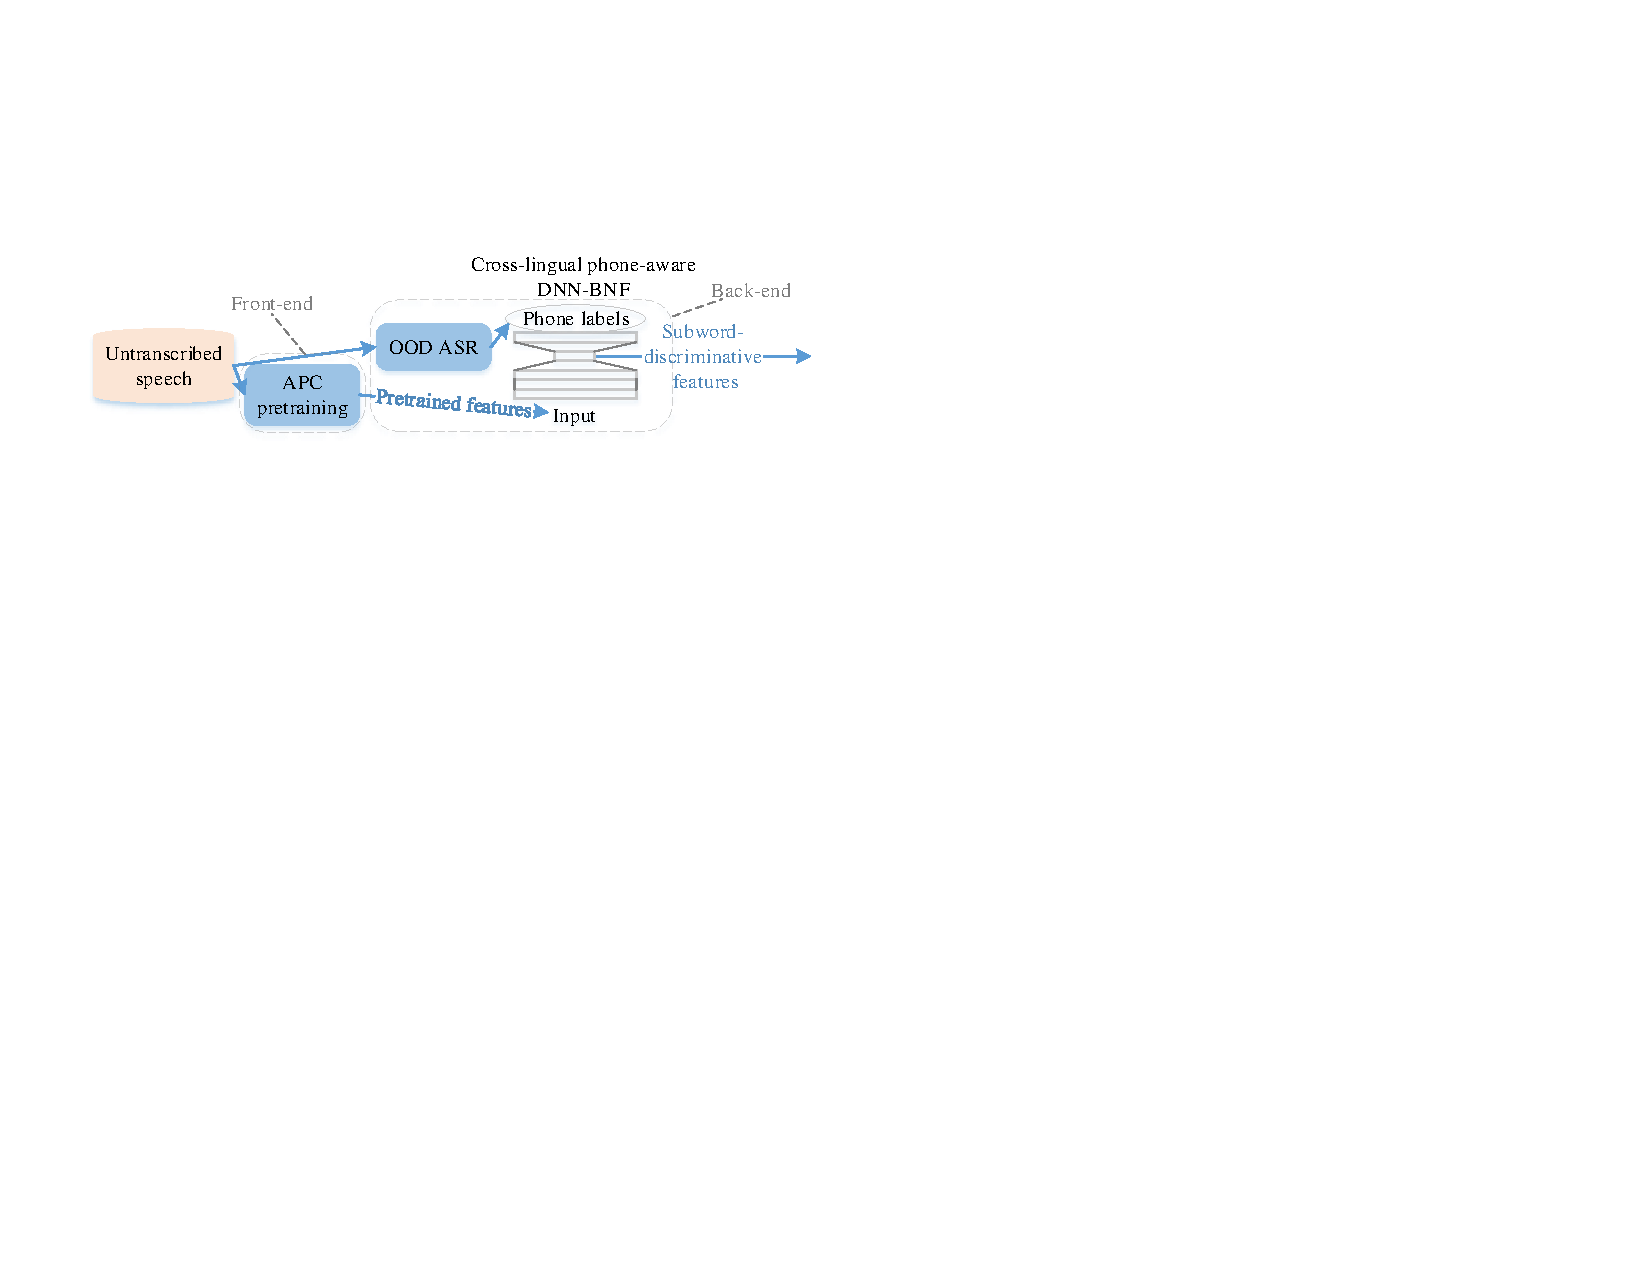
\includegraphics[width=\linewidth]{LaTeX/apc_framework_detail.pdf}
    \caption{General framework of the proposed approach to unsupervised subword modeling.  }
    \label{fig:general_framework}
\end{figure}
The general framework of our proposed approach is illustrated in Figure \ref{fig:general_framework}. Given untranscribed speech data of a    language, an APC  model is pretrained at front-end.
% stage.
% and used to extract pretrained features.
% is used to pretrain the data 
An OOD ASR system for a language different from the target language  assigns a phone label to every frame of the data. Pretrained features by the APC model and  cross-lingual phone labels are used to train a DNN-BNF model at back-end, from which BNFs are extracted as the subword-discriminative representation.
\subsection{APC pretraining}
\label{subsec:apc}
% APC is an unsupervised feature learning method \cite{Chung2019}. 
% It was proposed by \cite{Chung2019} to learn frame-level feature representation which facilitates a wide range of downstream tasks. 
The effectiveness of unsupervised APC pretraining  has been demonstrated in   ASR and SV tasks \cite{Chung2019}. This  indicates that APC could preserve both phonetic (subword) and speaker information in original speech, meanwhile the two types of information are more  separable and are more accessible to task-specific back-ends, comparing to spectral features and other feature learning methods \cite{Chung2019}. 

For our concerned unsupervised subword modeling task, previously adopted feature learning methods 
% such as FHVAE \cite{Feng2019improving} and adversarial training \cite{Higuchi2019} 
usually target suppressing speaker variation \cite{Feng2019improving,heck2017feature}. In contrast, the present study applies APC to learn a representation that keeps information in original speech, meanwhile phonetic information is made more separable to speaker information. The learned representation is considered less risky of losing phonetic information than \cite{Feng2019improving,heck2017feature}.
% expected to facilitate back-end subword-discriminative modeling, and is less risky of losing subword information.


% both subword and speaker information and they are more separable, hence facilitates back-end modeling to learn subword-discriminative representation of speech.%,  %The present study adopts APC to learn a feature representation

Let us assume a set of unlabeled training data $\{\bm{x_1}, \bm{x_2}, \ldots, \bm{x_T}\}$, where $T$ is the total number of frames. At each time step $t$, the encoder of APC model $\textrm{Enc}$ reads as input
$\bm{x_t}$, 
% $\bm{x_{1:t}}=\{\bm{x_1},\ldots,\bm{x_t}\}$ 
and outputs $\bm{y_t}$ (same dimension as $\bm{x_t}$) based on all the previous inputs $\bm{x_{1:t}}=\{\bm{x_1},\ldots,\bm{x_t}\}$,
\begin{equation}
    \bm{y_t} = \textrm{Enc} (\bm{x_{1:t}}).
    \label{eqt:enc}
\end{equation}
The goal of APC is to let $\bm{y_t}$ be as close to $\bm{x_{t+n}}$ as possible, where $n$ is a pre-defined constant positive integer, denoted as \textit{prediction step}. 
% In other words, an APC tries to predict a speech frame that is $n$ steps ahead of the current time. 
The loss function during APC   training is defined as: $\textrm{Loss} = \sum_{t=1}^{T-n} \left| \bm{y_t} - \bm{x_{t+n}} \right|$.
% \begin{equation}
%     \textrm{Loss} = \sum_{t=1}^{T-n} \left| \bm{y_t} - \bm{x_{t+n}} \right|.
%     \label{eqt:apc_loss}
% \end{equation}
% By minimizing the loss function in Equation (\ref{eqt:apc_loss}), the APC encoder can be trained.
Intuitively, increasing $n$ encourages the   encoder to capture contextual dependencies in speech, 
% more global structures in speech, 
while a small $n$ focuses more on local smoothness.
 
The encoder of APC is realized by the long short-term memory (LSTM) \cite{hochreiter1997long} RNN in this work. Let $L$ denote the number of LSTM layers,  Equation (\ref{eqt:enc}) is formulated as,
\begin{align}
    \bm{h_0} &= \bm{x_{1:t}},    \\
    \bm{h_l} &= \textrm{LSTM}^l (\bm{h_{l-1}}), l\in \{1,2,\ldots, L\}, \\
    \bm{y_t} &= \bm{W} \bm{h_L}.
\end{align}
Details of the  layer structure $\textrm{LSTM} (\cdot)$ can be seen in \cite{sak2014long}.

After APC training, the output of the top hidden layer $\bm{h_L}$ is extracted as the  learned  representation, and is referred to as \textit{APC features} in this paper. In principle,  $\bm{h_l}$ of any layer $l$ could be used as the learned representation. Results in \cite{Chung2019} suggest that outputs of higher layers  are more suitable for phone classification than lower layers. Following \cite{Chung2019} we choose to use the output of the top layer.
% , while lower layer outputs are  more suitable for speaker classification.
% Here $\bm{h_l}$ denotes the output of  

% , APC pretrained features surpass spectral features 
% which require 
% phonetic and speaker information in APC features are both more accessible to their respective back-end models for ASR and SV tasks.
% (-) Architecture of Enc.\\
% (-) how to extract features from APC to back-end.
% APC pretrained features  tend to retain as much information encoded in original speech representation as  possible. 
% different types of information in APC features, such as phonetic and speaker information, are both more accessible to the back-end models corresponding to their respective tasks.
\subsection{Cross-lingual phone-aware DNN-BNF}
% The back-end of our proposed approaches is t
% The DNN-BNF model  \cite{chen2017multilingual,feng2018exploiting} is adopted as the back-end of our proposed approach. 
As shown in Figure \ref{fig:general_framework}, the DNN-BNF back-end
% it 
is a DNN with a bottleneck   layer in the middle. BNFs could provide compact and subword-discriminative representation  \cite{grezl2009investigation}.  
% Training of a subword-discriminative DNN-BNF model requires frame labels \cite{chen2017multilingual}. 
In the zero-resource scenario, phone labels  required for DNN-BNF modeling are not directly available.
% cannot be obtained due to the absence of transcriptions. 
This study leverages an OOD language-mismatched ASR system to generate cross-lingual phone labels for target  speech.
{\color{blue}The motivation  is that
% Although languages vary greatly in pronunciation, 
speech sounds in different languages are believed to have much overlap at phone level.}
To obtain cross-lingual labels, the OOD ASR is used to decode  and find the best paths for  target speech utterances. Through decoding, each speech frame is assigned with a triphone HMM state modeled by the OOD ASR. These phone labels provide phonetic representation for the target speech from a cross-lingual perspective. 

% It is worth noting that decoding results depend on the relative weighting  of the ASR AM and language model (LM). In this study, the LM carries a very small weight, in order to ensure decoding results mainly reflect acoustic characteristics of target speech.

After obtaining cross-lingual  phone labels, the DNN-BNF can be trained in a supervised manner \cite{grezl2007probabilistic}, and used to  extract BNFs   as the subword-discriminative feature representation. 
% The cross-lingual HMM labels are used as supervision for in-domain speech data in DNN-BNF modeling.
% After obtaining cross-lingual  HMM state labels, a DNN-BNF model is trained with target speech, using these labels as supervision.  
% The DNN-BNF is trained to optimize cross-lingual phone classification accuracy.
The input features to DNN-BNF are APC features. 
% After training, the DNN-BNF is used to extract BNFs for target speech as the subword-discriminative feature representation. 
The choice of language identities of OOD ASR systems is flexible in principle. 
In the present study, OOD ASR systems for two different languages are utilized to generate phone labels. They are compared in the experiments.
% to generate cross-lingual labels, in order to study the effect  of OOD  language identities on unsupervised subword modeling.
% its influence towards the final performance.
% our proposed approaches.

% (-) OOD ASR decoding\\
% (-) DNN-BNF training with APC features and cross-lingual phone labels\\
% (-) Effect of OOD language identity.
% Authors should observe the following rules for page layout. A highly recommended way to meet these requirements is to use a given template (Microsoft Word?? or LaTeX) and check details against the corresponding example PDF file. Given templates, Microsoft Word\textregistered\ or \LaTeX, can be adapted/imported easily in other software such as LibreOffice, Apple Pages, Lua\LaTeX, and Xe\LaTeX, but please be careful to match the layout of the provided PDF example.

\section{Experimental setup}

\subsection{Databases and evaluation metric}
Experiments in this study are carried out on two databases: Libri-light \cite{kahn2019librilight} and ZeroSpeech 2017 \cite{dunbar2017zero}. Libri-light is a newly published   database to facilitate research on ASR under limited or zero resource scenarios. It is by far the largest public database to support evaluation on unsupervised subword modeling. The language in Libri-light is English. The \texttt{unlab-600} set from Libri-light is adopted as training data in most of our experiments. This set contains 
% $36,229$ utterances by $489$ speakers, summing up to
in total $526$ hours of speech. In addition, we randomly select subsets of utterances in unlab-600   to form smaller-sized training sets. There are four smaller-sized training sets constructed in this study, with the numbers of utterances ranging from $900$ to $3.6$K, $7.2$K and $14.4$K. In addition, \texttt{unlab-6K} is adopted in part of the experiments. Details of the training sets are summarized in Table \ref{tab:libri_light_data}.
\begin{table}[!tbp]
\renewcommand\arraystretch{1}
\centering
\caption{Libri-light training data and its subsets.}
\resizebox{1 \linewidth}{!}{%
\begin{tabular}{l|cccccc}      
% \hline      
% \toprule
Name&unlab-6K& unlab-600 & sub14.4K & sub7.2K & sub3.6K & sub0.9K \\
%  & \multicolumn{3}{c|}{ Training} & Test \\
\midrule
\#utterances &$362,817$ &  $36,229$ & $14,400$ &$7,200$ &$3,600$ &$900$ \\
\#speakers & $1,742$ & $489$ & $438$ & $393$ & $351$ & $244$ \\
Hours & $5,273$ &$526$& $209$ & $104$ & $52$ & $13$ \\
%  & Duration  &\#speakers-R\tablefootnote{``speakers-R/-L'' denotes speakers with rich/limited speech data.} &\#speakers-L\footnotemark[1]  & Duration\\
% \hline
% \midrule

% Training hours:  & $19.3$ & $81.5$ & $105.3$ \\
% Test hours:& $0.6$ & $0.7$ & $5.9$ \\
% Basic acoustic unit:  & Phone & Phone & Initial-Final \\
% \#basic units (inc. sil):& $33$ & $87$ & $61$ \\
% \#tied CD-HMM states:& $2462$ & $3431$ & $2386$ \\ 
% Lexicon size:& $ $ & $ 133K$& $ $ \\
% $\#$ Phonemes: &$43$& $46$&$ 29$& $44$& $38$\\
% \hline
% \bottomrule
\end{tabular}%
% \footnotetext{`speakers-R/-L' denotes speakers with rich/limited speech data}
}
\label{tab:libri_light_data}
\end{table}
The evaluation data in Libri-light consists of four sets, \textit{dev-clean, dev-other, test-clean} and \textit{test-other}. 
They are identical to the sets in Librispeech database \cite{panayotov2015librispeech}. 

ZeroSpeech 2017 database is   used in our experiments only for the purpose of performance evaluation. The English test set in ZeroSpeech is adopted, as our system is trained with English unlabeled data. 
% contains three languages, English, French and Mandarin. In our experiments, ZeroSpeech training data is not used, and 
% Our systems are trained solely on Libri-light. ZeroSpeech evaluation data for English is used. 
The test set is organized into subsets of differing   lengths (1s, 10s and 120s)  \cite{dunbar2017zero}.
% consists of three utterance length settings, $1$s
% English 


The evaluation metric is  ABX subword discriminability \cite{dunbar2017zero}.
In the ABX task, $A$, $B$ and $X$ are three speech segments, $x$ and $y$ are two different phonemes. $A \in x$, $B \in y$, $X \in x$ or $y$. An error occurs if under a pre-defined distance measure $d$, $d(A,X) > d(B,X)$, given $X \in x$, 
or $d(A,X) < d(B,X)$, given $X \in y$.
% and vice versa.
% is to decide whether $X$ belongs to $x$ or $y$ if $A$ belongs to $x$ and $B$ belongs to $y$, where $A$, $B$ and $X$ are three speech segments, $x$ and $y$ are two different phonemes. 
% each consisting of $3$ consecutive phonemes (e.g. \quotes{b-e-g}). 
% $x$ and $y$ are two different phonemes. By saying $X$ belongs to $x$, it means the central phoneme in $X$ is $x$. 
Details of  ABX error rate computation can be found in \cite{dunbar2017zero}, where dynamic time warping is chosen as the distance measure. Segments $A$ and $B$   belong to the same speaker. ABX error rates for \textit{within-speaker} and \textit{across-speaker} are evaluated separately, depending
on whether X and A(B) belong to the same speaker.
% A low ABX error rate is preferable as it indicates  the feature representation is good at distinguishing subword units. 
% Each pair of $A$ and $B$ are generated by the same speaker. 
% ABX error rates for \textit{within-speaker} and \textit{across-speaker} are evaluated separately, depending on whether $X$ and $A(B)$ belong to the same speaker. Software to compute ABX error rates on Libri-light and ZeroSpeech are both provided by their developers.
\subsection{APC and comparing method}
\label{subsec:exp_setup_apc_fhvae}
The APC model is implemented as a  multi-layer  LSTM network. Residual connections are made between two consecutive layers.  
Each LSTM layer has $100$ dimensions.
Unless specified, the number of LSTM layers is $3$.
The prediction step $n$ (in Section \ref{subsec:apc}) is set to  the optimal value within $\{1,2,3,4,5\}$. Our preliminary experiments showed that $n$ larger than $5$ would lead to rapid degradation in ABX error rate. 
The input features to APC are $13$-dimension MFCC with cepstral mean normalization (CMN) at speaker level. 
The model is trained for $100$ epochs using the Adam optimizer \cite{kingma2014adam}, with an initial learning rate of $10^{-4}$. The batch size is  $32$. An open-source tool by \cite{Chung2019} is used to train the APC model. 
% MFCC features are extracted by Kaldi \cite{povey2011kaldi}. 
After training, the top LSTM layer's output is extracted as APC features.

FHVAE was previously adopted \cite{Feng2019improving} as the front-end to address the same problem as in this study. Its latent representation $\bm{z_1}$ is known of preserving linguistic content while suppressing speaker variation \cite{hsu2017nips}. Here, $\bm{z_1}$ is used to make comparison with the APC feature. The model architecture of FHVAE and its training procedure follow the settings in \cite{Feng2019improving}.
The input feature representation is the same for FHVAE and  APC. FHVAE training is implemented using an open-source tool \cite{hsu2017nips}. Both FHVAE and APC are trained with Libri-light. 
 % Encoder structure, LSTM no. layers, input data size, $n$ is tuned. epochs, learning rate, batch size
\subsection{OOD ASR systems}
There are two OOD ASR systems employed in our experiments. The first one is a Dutch ASR trained with CGN \cite{oostdijk2000spoken}, a transcribed speech corpus covering  speaking styles including conversations, read speech, broadcast news (BN), etc.
% Speech spoken by people in the Netherlands are used. 
The training and test data partition follows \cite{laurensw75cgn_kaldi}. The training data comprises $483$
 hours of speech. A chain-time delay NN (TDNN) AM \cite{povey2016purely} is trained by Kaldi. It contains $7$ TDNN layers. The input features are $40$-dimension high-resolution (HR) MFCCs. 
%  Training data are speed perturbed with scales $0.9, 1.0$ and $1.1$, making the actual  amount of training data tripled. 
 The TDNN AM is trained based on lattice-free maximum mutual information (LF-MMI) criterion \cite{povey2016purely}. Frame labels required for TDNN training are generated by forced-alignment with a GMM-HMM AM trained beforehand. The number of modeled Dutch phones is $81$ (including a silence phone).
 A tri-gram LM is trained using training data transcriptions. 
The Dutch ASR reports $8.98\%$ word error rate (WER) on the CGN BN test set.

The second OOD ASR system is a Mandarin ASR trained with Aidatatang\_200zh, a read speech corpus developed by \cite{aidatatang}. The training set comprises $140$ hours of speech. 
% A chain-TDNN AM is trained. 
The AM for Mandarin ASR has a similar architecture with the Dutch AM mentioned above. The differences are: HR MFCC input  features are further appended by $3$-dimension pitch features \cite{ghahremani2014pitch}; the number of modeled Mandarin phones is $119$ (including a silence phone). 
A tri-gram LM is trained using training data transcriptions.
The Mandarin ASR reports $6.37\%$ character error rate (CER) on Aidatatang\_200zh test set.

%  ; Speech by people from the Netherlands are used; This corpus comprises conversations, interviews, lectures, debates, read speech and broadcast news. Training and test data partition follows \cite{laurensw75cgn_kaldi}
% Training: $483$ hours, chain model, 
% TDNN, layer structure, input features, $81$ modeled phones (including a silence phone), $3,488$ triphone HMM states.
% gives WER $8.98\%$ on broadcast news test set. 

% Mandarin ASR trained with Aidatatang\_200zh \cite{aidatatang}
% Training data contains $140$ hours speech, read speech, TDNN model, input is MFCC plus pitch, $119$ modeled phones (including a silence phone), $4,400$ triphone HMM states , CER $6.37\%$ on test set. 
\subsection{DNN-BNF setup}
DNN-BNF models are trained using Libri-light (English) training data and cross-lingual phone labels. 
One DNN-BNF  is trained with phone labels generated by the Dutch ASR, while the other DNN-BNF is trained with labels by the Mandarin ASR. To obtain Dutch or Mandarin frame labels for English training data,  HR MFCC features (and appended by pitch features if to obtain Mandarin labels) of Libri-light are extracted, and fed as inputs to the Dutch/Mandarin ASR system for decoding. 
During decoding, the LM to AM weight ratio is set to $0.001$.
The decoding results, i.e. word transcriptions,  are  forced-aligned by the Dutch/Mandarin AM to generate HMM state alignments\footnote{Here \textit{alignment} is slightly different from the `norm', as it contains alternative pronunciations. This is required by chain model training of DNN-BNF in Kaldi.} as frame labels.

The DNN-BNF consists of $7$ feed-forward layers with ReLU activation. Each layer has $450$ dimensions except a $40$-dimension BN layer at the second top. The DNN-BNF is implemented  as a chain model in Kaldi. The training procedure  is based on  LF-MMI criterion. 
The inputs to DNN-BNF are APC  features with contextual splicing $\{0,\pm 1\}$.
Training labels are either Dutch  or Mandarin frame labels. After DNN-BNF training, $40$-dimension BNFs are extracted as the learned subword-discriminative representation and evaluated by the ABX task.
% of target speech. 

% and phonetic-alignments in Dutch/Mandarin. 
% One could directly obtain frame labels from phonetic-alignments. However we rely on transcriptions to be aligned by Dutch/Mandarin AM. Just for practical consideration, as DNN-BNF is under Kaldi nnet3 recipe, 
%[kaldi chain model numerator FST]Instead of enforcing a particular pronunciation of the training data, we use as our reference a lattice of alternative pronunciations of the training data, generated by a lattice-generating decoding procedure using an utterance-specific graph as the decoding graph. This generates all alignments of pronunciations that were within a beam of the best-scoring pronunciation.



The DNN-BNF model could also be trained using conventional spectral features as inputs. 
In such case, DNN-BNF training keeps the same as mentioned above, except that input features are $40$-dimension HR MFCCs with the same contextual splicing. After DNN-BNF training, the resulting BNFs are also evaluated by the ABX task.
% BNF representation is   extracted.
% as a reference.
% including cross-lingual phone labeling, and DNN-BNF training.

\section{Results and discussion}
\subsection{Effectiveness of APC features }

ABX error rates ($\%$) of  APC features  and FHVAE features ($\bm{z_1}$, mentioned in Section \ref{subsec:exp_setup_apc_fhvae}) with respect to different amount of training data are shown in Figure \ref{fig:apc_fhvae_mfcc}.
{\color{blue}
In this subsection, APC  features and $\bm{z_1}$ are directly evaluated by the ABX task, without being modeled by the  DNN-BNF back-end. The performance comparison is made at front-end.}
\begin{figure}[!t]
    \centering
    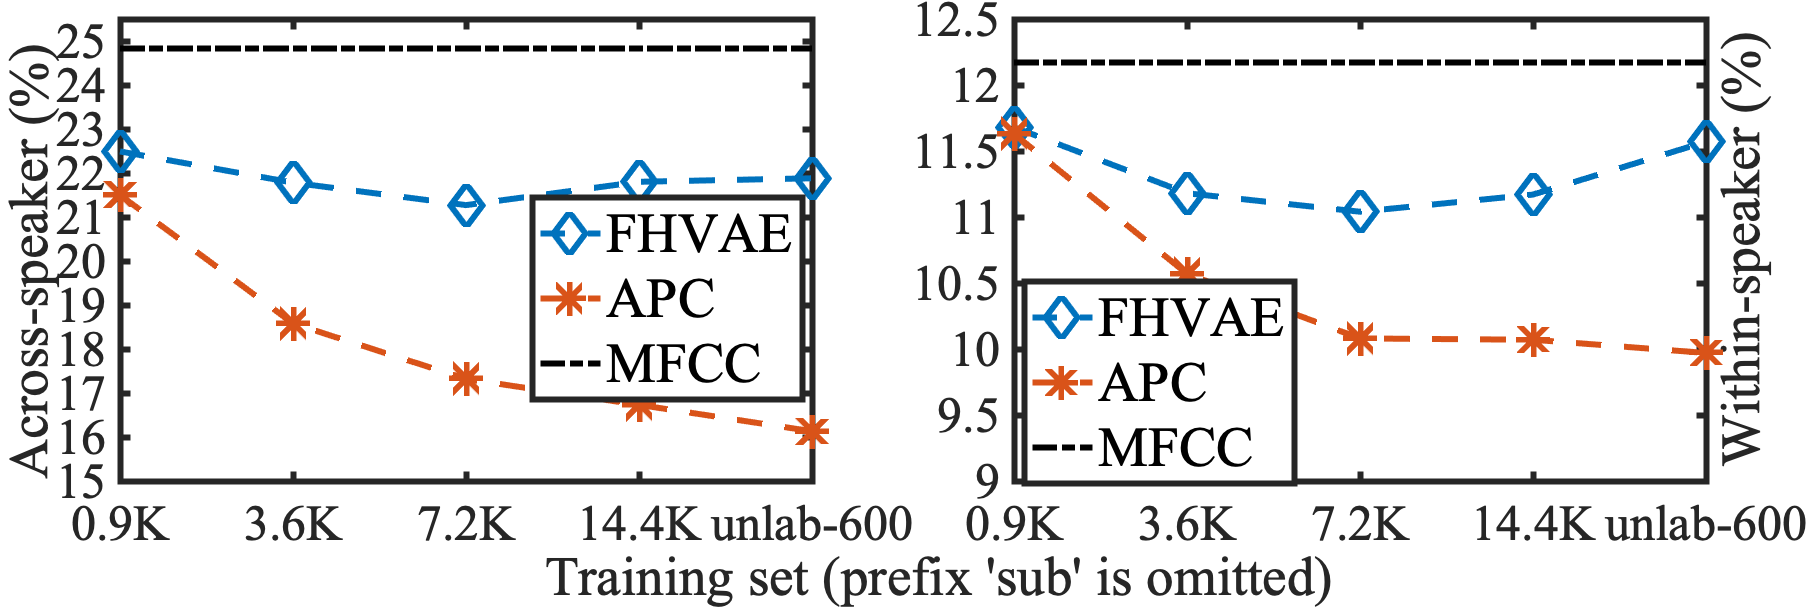
\includegraphics[width=.9\linewidth]{LaTeX/apc_fhvae_mfcc_no_sub.png}
    \caption{ABX error rate  of features learned by APC, FHVAE and official MFCC baseline on Libri-light (Avg. over $4$ sets). }
    \label{fig:apc_fhvae_mfcc}
\end{figure}
% these two features are learned without performing DNN-BNF modeling. 
ABX results in  Figure \ref{fig:apc_fhvae_mfcc} are averaged values over the $4$ evaluation sets in Libri-light. The official MFCC baseline   \cite{kahn2019librilight} is also shown in this Figure. It can be observed that both APC features and $\bm{z_1}$  outperform MFCC features. The APC features are consistently superior to $\bm{z_1}$ in all the training data amount settings ($13 \sim 526$ hours, i.e. sub0.9K to unlab-600). 
While APC model is not aimed explicitly at suppressing speaker variation as FHVAE is,   
Figure \ref{fig:apc_fhvae_mfcc} (left) indicates that APC features are more effective than   $\bm{z_1}$ in distinguishing subword units across different speakers.

% (-) a curve showing ABX error rate of APC features, FHVAE latent segment variables and MFCC features w.r.t training data amount.

\subsection{Effectiveness of BNF representation}
\begin{table}[!t]
\renewcommand\arraystretch{0.80}
\centering
\caption{ABX error rate of  BNFs, APC and CPC features  on Libri-light. Models are trained with unlab-600. `Du' and `Ma' stand for Dutch and Mandarin. APC encoder has $5$ layers.}
\resizebox{0.95 \linewidth}{!}{%
\begin{tabular}{l|cc|cccc|c}      
% \hline      
\toprule
\midrule[0.2pt]
& \multicolumn{7}{c}{Across-speaker}\\
Feature&Input & Label & dev-clean & dev-other & test-clean & test-other & Avg.\\ 
\midrule
%  & \multicolumn{3}{c|}{ Training} & Test \\
\multirow{4}{*}{BNF} &APC & Du & $\bm{6.18}$&	$\bm{11.02}$&$	\bm{6.03}$	&$\bm{10.94}$&$	\bm{8.54}$\\
&MFCC & Du &$6.67$&$	11.65$&	$6.64$&$	12.00$&$	9.24$\\
&APC & Ma & $7.00$&$11.80$&$6.84$&$11.81$&$9.36$\\
% &APC & Ma & $6.89$&	$11.83$&	$6.82$&	$11.78	$&$9.33$\\
&MFCC & Ma & $7.92$&	$12.71$&	$7.74$&	$13.23$&	$10.40$\\
\midrule
APC& -&- & $12.64$&$	19.00$&$12.19$&$18.75$&$15.65$\\
CPC \cite{kahn2019librilight} & -&-&$9.58$&	$14.67$&	$9.00$&	$15.10$&	$12.09$\\
% \midrule


\midrule
&\multicolumn{7}{c}{Within-speaker} \\
% Input & Label & dev-clean & dev-other & test-clean & test-other & Avg.\\ 
\midrule
\multirow{4}{*}{BNF} &APC & Du  & $\bm{4.77}$&	$\bm{6.69}$&	$\bm{4.49}$&	$\bm{6.43}$&	$\bm{5.60}$\\
&MFCC & Du & $4.97	$&$6.94$&	$4.73$&	$6.86$&	$5.88$\\
&APC & Ma  & $5.25$&	$7.14$&	$5.21$&	$7.09$&	$6.17$\\
&MFCC & Ma & $6.06$&	$7.71$&	$5.62$&	$7.82$&	$6.80$\\
\midrule
APC&-& -& $8.83$&$11.07$&$8.36$&$11.48$&$9.94$\\
CPC \cite{kahn2019librilight}&-&- &$7.36$&	$9.39$&	$6.90$&	$9.59$&	$8.31$\\
% &dev-clean & dev-other & test-clean & test-other  \\
\midrule[0.2pt]
\bottomrule
\end{tabular}%

}
\label{tab:dnn_bnf}
\end{table}
ABX error rates (\%) of BNFs extracted from  DNN-BNF are listed in Table \ref{tab:dnn_bnf}. The second and third columns  denote input feature types and frame labels for training DNN-BNF models.
The performance  of    APC  and CPC features (by \cite{kahn2019librilight}) are also listed for reference. {\color{blue}APC and CPC are   not modeled by the DNN-BNF back-end.}
% Note that the APC model in Table \ref{tab:dnn_bnf} consists of $5$ LSTM layers instead of $3$. 
All the models are trained with unlab-600.   From this Table, it is observed  that:

(1) DNN-BNF trained with APC features performs better than that trained with MFCC features in all evaluation sets. This  demonstrates the effectiveness of front-end APC pretraining in our proposed two-stage system framework.

(2) BNF outperforms the front-end APC  feature to a large margin. 
% The  BNF trained with  Dutch phone labels  achieves $45\%$ and $44\%$ relative error rate reduction over APC features in across- and within-speaker test conditions. 
% For DNN-BNF models trained with Mandarin labels, similar observation is   made. 
The results show that back-end DNN-BNF modeling with cross-lingual phone labels
% leveraging OOD language resources 
could significantly improve unsupervised subword modeling. This observation is shared with previous works \cite{shibata2017composite,feng2019_TASLP}. BNF also performs better than the   CPC feature    \cite{kahn2019librilight}. Note that \cite{kahn2019librilight} does not leverage OOD resources.

(3) The performance achieved by adopting Dutch labels in DNN-BNF modeling is slightly better than that by adopting Mandarin labels. 
% ($9.33\%/6.17\%$). 
This could be interpreted by the similarity between the OOD language and target in-domain language. Dutch and English are both West Germanic languages. Their similarity is believed to be stronger than Mandarin and English. While the Dutch ASR  is trained with more data ($483$ hours) than the Mandarin ASR ($140$ hours), the evaluation results on their respective in-domain test sets (Dutch: $8.98\%$ WER; Mandarin: $6.37\%$ CER) indicate that their performance does not differ much.

% their in-domain ASR performance (Dutch: $8.98\%$ WER; Mandarin: $6.37\%$ CER) do not differ much. 


%reveals the effect of the OOD language identity
% \begin{enumerate}
%     \item d
% \end{enumerate}

% (-) this part will give table to list results in detail. Table showing unlab-600 results. 

% Our proposed approaches best performance $8.54\%$ and $5.60\%$. 

% DNN-BNF with APC features better than that with MFCC features. 
% Mandarin labels slightly inferior to Dutch labels. 
% Probably is explained by language similarity English-Dutch is stronger than English-Mandarin. 
% Results better than CPC \cite{kahn2019librilight}, a purely unsupervised approach without leveraging OOD resources.

% (-) Need to mention in this part, APC encoder has $5$ LSTM layers instead of $3$.

% (-) May also draw observations between comparing Dutch labels and Mandarin labels. THen next subsection focuses on sensitivity of training data amount
% DNN-BNF trained with Dutch labels is discussed. Mandarin labels will be included in the next subsection. 

\subsection{Effect of  training data amount}
\begin{figure}[!t]
    \centering
    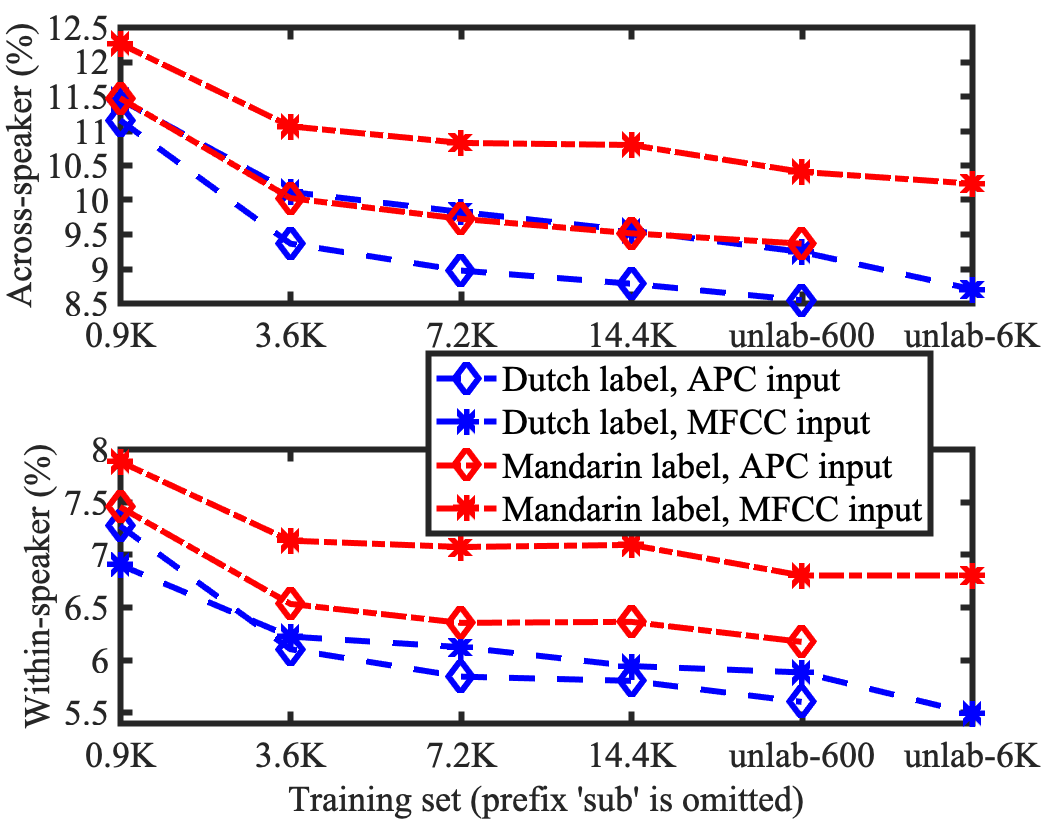
\includegraphics[width=0.71\linewidth]{LaTeX/crsling_dnn_bnf_apc_input_vert_no_prefix_adt_apc_across_9.36.png}
    \caption{ABX error rate of BNFs w.r.t training data amount on Libri-light (Avg. over $4$ sets).}
    \label{fig:dnn_bnf_data_amount}
\end{figure}
ABX error rates ($\%$) of BNFs extracted by  DNN-BNF models with respect to different amount of training data are illustrated in Figure \ref{fig:dnn_bnf_data_amount}. The results are averaged values over the $4$ evaluation sets in  Libri-light. \texttt{Unlab-6K}  is  adopted for DNN-BNF models with MFCC inputs (marked as `$\ast$'). For models trained with APC features (marked as `$\diamond$'), the training set for DNN-BNF modeling and for APC pretraining keeps the same. From Figure \ref{fig:dnn_bnf_data_amount}, it is clearly seen that 
% increasing the amount of training data leads to better ABX performance. 
% When training data increases from $13$ hours to $52$ hours, 
the improvement is more dramatic when training data increases from $13$  hours (sub0.9K) to $52$ hours (sub3.6K), compared to   that from $52$ hours to over $500$ hours (unlab-600). 

DNN-BNF models trained with APC features as input features are almost consistently better than models with MFCC input features in different training data amount settings. 
In particular, using Dutch labels,  the model trained with APC features with the  sub14.4K set achieves similar across-speaker error rate ($8.78\%$)  to the model trained with MFCCs with the unlab-6K set ($8.71\%$). This implies  APC pretraining saves training data amount from over $5,000$ hours to around $200$. This is highly appealing in low-resource speech modeling. When Mandarin labels are used for DNN-BNF modeling, APC pretraining  could save even more training data amount without ABX error rate degradation. 
% In real-world applications, it is sometimes impractical to gain knowledge on language similarity between the target unknown language and resource-rich languages. 
% APC pretraining 
% From this perspective,
% Mandarin phone labels are less ideal to English speech than Dutch ones, making DNN-BNF input feature quality more essential.
% The benefit of data increase is twofold: improvement on APC features
% This set comprises $5.3$K hours of speech, roughly tenfold of unlab-600.


% compare results of dnn-bnfs with Dutch ASR labels and Mandarin ASR labels.
% Will show as Figure  \ref{fig:dnn_bnf_data_amount}. 
% Will have to introduce unlab-6K set.
% Need to explain in Figure \ref{fig:dnn_bnf_data_amount}
% , for systems with APC features as input, the training set used in APC pretraining and DNN-BNF modeling is always the same.

% (-) Increasing from 10+ hours to 50+ hours gives prominent performance improvement. from 50+ hours to 500+ hours the improvement still there but more gradual.

% (-) By applying APC pretraining, DNN-BNF consistently outperform that w/o APC. Particularly most cases, w/ APC at 522h more effective than w/o APC but at 5.2K h.


% \section{Discussion}
\subsection{ZeroSpeech 2017 results}
\begin{table}[!t]
\renewcommand\arraystretch{0.80}
\centering
\caption{ABX error rate of  BNFs  on ZeroSpeech 2017 English sets. Models are trained with  Libri-light using Dutch labels.}
\resizebox{1 \linewidth}{!}{%
\begin{tabular}{cl|ccc|c|ccc|c}      
% \hline      
\toprule
\midrule[0.2pt]
& &\multicolumn{4}{c|}{Across-speaker}& \multicolumn{4}{c}{Within-speaker}\\
System &   Train set & 1s & 10s & 120s & Avg. &1s &10s &120s &Avg.\\
\midrule[0.2pt]

\multirow{ 3}{*}{Proposed} & unlab-600  & $7.65$&$6.69$&$6.66$&$\bm{7.00}$&$5.52$&$4.77$&$4.68$&$\bm{4.99}$\\
& sub14.4K & $8.11$&$6.99$&$6.90$&$7.33$&$5.83$&$5.06$&$4.97$&$5.29$\\
& sub7.2K & $8.14$&$7.07$&$7.03$&$7.41$&$5.89$&$4.99$&$5.00$&$5.29$ \\
\midrule[0.2pt]
Topline \cite{dunbar2017zero}&  &$8.6$&$6.9$&$6.7$&$7.40$ &$6.5$&$5.3$&$5.1 $&$5.63$\\
  \cite{shibata2017composite}& & $7.9$&$7.4$&$6.9$&$7.40$&$5.5$&$5.2$&$4.9$&$5.20$\\
% \midrule
% \midrule
% \multicolumn{5}{c}{Within-speaker} \\
% \midrule[0.2pt]
%  unlab-600  & \\
%  sub14.4K & \\
% \ Topline \cite{dunbar2017zero}   &$6.5$&$5.3$&$5.1 $&$5.63$\\
% &dev-clean & dev-other & test-clean & test-other  \\
\midrule[0.2pt]
\bottomrule
\end{tabular}%

}
\label{tab:zrsc2017}
\end{table}
The performance of our approach evaluated on ZeroSpeech 2017 English sets is listed in Table \ref{tab:zrsc2017}. The official topline \cite{dunbar2017zero}  and the best-performing system (using OOD data) \cite{shibata2017composite} are also listed. The topline and \cite{shibata2017composite}  employed English labeled data while our models do not. The total number of hours of labeled training data used in \cite{shibata2017composite} is $1,327$ (including $80$-hour English data).
Our system trained with unlab-600 outperforms topline and \cite{shibata2017composite}, and is comparable to the two reference systems when trained with sub7.2K ($104$ hours).
% The system \cite{shibata2017composite} is best-performing.

% report our results and 
% supervised topline, as well as 
% recent papers benchmarked here, \cite{riviere2020unsupervised} used Librispeech-360 to train CPC;
% \cite{shibata2017composite} best system used 10 languages including English labeled data; 
% \cite{chorowski2019unsupervised} used ZRSC training data only.

\section{Conclusions}
This study addresses unsupervised subword modeling, and proposes a two-stage system that consists of APC pretraining and cross-lingual phone-aware DNN-BNF modeling.  
Experiments are carried out on Libri-light and ZeroSpeech 2017 databases and evaluated by the ABX task. Experimental results confirm the effectiveness of APC in front-end feature pretraining. It surpasses a previously adopted FHVAE approach. Our whole system outperforms the state of the art in both databases. The proposed approach benefits from increasing training data amount, and is less sensitive to data amount when the training data is over $50$ hours. APC pretraining could save  data amount from over $5,000$ hours to around $200$ hours for the proposed system without performance degradation in across-speaker ABX error rate.  
Cross-lingual phone labeling for English data by a Dutch ASR is slightly better than by a Mandarin ASR. This could be explained as the stronger similarity between English and Dutch.  

% \section{Acknowledgements}




\bibliographystyle{IEEEtran}

\bibliography{mybib}

% \begin{thebibliography}{9}
% \bibitem[1]{Davis80-COP}
%   S.\ B.\ Davis and P.\ Mermelstein,
%   ``Comparison of parametric representation for monosyllabic word recognition in continuously spoken sentences,''
%   \textit{IEEE Transactions on Acoustics, Speech and Signal Processing}, vol.~28, no.~4, pp.~357--366, 1980.
% \bibitem[2]{Rabiner89-ATO}
%   L.\ R.\ Rabiner,
%   ``A tutorial on hidden Markov models and selected applications in speech recognition,''
%   \textit{Proceedings of the IEEE}, vol.~77, no.~2, pp.~257-286, 1989.
% \bibitem[3]{Hastie09-TEO}
%   T.\ Hastie, R.\ Tibshirani, and J.\ Friedman,
%   \textit{The Elements of Statistical Learning -- Data Mining, Inference, and Prediction}.
%   New York: Springer, 2009.
% \bibitem[4]{YourName17-XXX}
%   F.\ Lastname1, F.\ Lastname2, and F.\ Lastname3,
%   ``Title of your INTERSPEECH 2020 publication,''
%   in \textit{Interspeech 2020 -- 20\textsuperscript{th} Annual Conference of the International Speech Communication Association, September 15-19, Graz, Austria, Proceedings, Proceedings}, 2020, pp.~100--104.
% \end{thebibliography}

\end{document}
